\documentclass[16pt]{beamer}
\usepackage{algorithm}
\usepackage{algorithmic}
\usepackage[numbers]{natbib}
% \usepackage{beamerthemesplit} // Activate for custom appearance

\title{The Sequence Memoizer}
\author{Frank Wood \\\qquad \\ joint work with Nicholas Bartlett, Jan Gasthaus, C\'{e}dric Archambeau, Lancelot James, Yee Whye Teh}
\date{\today}



\usetheme{Darmstadt}
%\usetheme{Copenhagen}
%\usefonttheme[onlylarge]{structurebold}
%\setbeamerfont*{frametitle}{size=\normalsize,series=\bfseries}
%\setbeamertemplate{navigation symbols}{}

\usepackage{amsfonts}
\usepackage{amsmath}
%\newcommand{\argmax}{\operatornamewithlimits{argmax}}
\def\newblock{\hskip .11em plus .33em minus .07em}
% Setup TikZ

\newcommand{\ubf}{\mathbf{u}}
\newcommand{\xbf}{\mathbf{x}}
\newcommand{\sbf}{\mathbf{s}}
\newcommand{\py}{\mathcal{PY}}
\newcommand{\vbf}{\mathbf{v}}
\newcommand{\Prob}{\mathrm{P}}
\newcommand{\Psmooth}{\Prob_\text{smooth}}
\newcommand{\parent}{\pi}
\newcommand{\suffix}{\sigma}
\newcommand{\UHPYP}{SM}
\newcommand{\PLUMP}{PLUMP}
\newcommand{\Oh}{\mathcal{O}}
\newcommand{\tree}{\mathcal{T}}

% \newcommand{\cusk}{c_{\ubf s k}}
% \newcommand{\cus}{c_{\ubf s \cdot}}
% \newcommand{\cu}{c_{\ubf \cdot \cdot}}
% \newcommand{\tus}{t_{\ubf s}}
% \newcommand{\tu}{t_{\ubf \cdot}}
\newcommand{\cusk}{c_{\ubf s k}}
\newcommand{\cus}{c_{\ubf s}}
\newcommand{\cu}{c_{\ubf \cdot}}
\newcommand{\tus}{t_{\ubf s}}
\newcommand{\tu}{t_{\ubf \cdot}}
\newcommand{\cset}{\{\cusk\}_{s\in \Sigma,k \in \{1,\ldots,t_{\ubf s}\}}}
\newcommand{\tset}{\{\tus\}_{s\in \Sigma}}
\newcommand{\bydef}{\equiv}
\newcommand{\state}{\mathcal{S}_{\xbf}}
\newcommand{\statei}{\mathcal{S}_{\xbf_{1:i}}}
\newcommand{\emptystring}{\varepsilon}
\newcommand{\gcount}{\hat{c}}
\newcommand{\escape}{\mathtt{esc}}

\newcommand{\todo}[1]{\begin{center}\textbf{TODO: } #1 \end{center}}
\newcommand{\figref}[1]{\figurename~\ref{#1}}
\newcommand{\predictive}{\Prob(x_i|\xbf_{1:i-1})}
\newcommand{\ywcomment}[1]{\textbf{#1}}
\newcommand{\jgcomment}[1]{ { \textcolor{red}{#1} } }




\title[Sequence Memoizer] 
{
	The Sequence Memoizer
}

\author[http://www.stat.columbia.edu/$\sim$fwood]
{
  Frank~Wood \\ 
 \qquad \\
  {\small joint work with \\ \qquad \\Y.W. Teh, N. Bartlett, J. Gasthaus, L. James, C. Archambeau}
}

\institute[Columbia University]
{
  %\inst{1}%
  Columbia University
}

%\def\blfootnote{\xdef\@thefnmark{}\@footnotetext}

% The main document

%\setbeamertemplate{framefooter}{ 
%\begin{centering} 
%\large{\insertframetitle} \\
%\small{\insertframesubtitle}
%\par 
%\end{centering} 
%} 


\begin{document}

\frame{\titlepage}

%\section[Outline]{}
%\frame[t]{\tableofcontents}
\section{Setup}
\subsection{Sequential discrete observations from an arbitrary stochastic process}
\frame[t]{
%\frametitle{Sequential Discrete Observations}
\begin{block}{Byte Sequence}
\[
\begin{array}{l}
01001001 , 01101110 , 00100000 , 01110100,\\
01101000 , 01110010 , 01100101 , 01100101,\\
00100000 , 01100100 , 01100001 , 01111001,\\
01110011 , 00100000 , 01111001 , 01101111,\\
01110101 , 01110010 , 00100000 , 01101000,\\
01100001 , 01110010 , 01100100 , 00100000,\\
01100100 , 01110010 , 01101001 , 01110110,\\
01100101 , 00100000 , 01110111 , 01101001,\\
01101100 , 01101100 , 00100000 , 01100011,\\
01110010 , 01100001 , 01110011 , 01101000\ldots
\end{array}
\]
\end{block}

\begin{block}{Binary Sequence}
\[
\begin{array}{l}
0,1,0,0,1,0,0,1...
\end{array}
\]
\end{block}
}


\subsection{``Black-box'' model desiderata and assumptions}
\begin{frame}[t]{}
Desiderata
\begin{itemize}
\item Incrementally estimate a {\em joint} distribution over sequences of unbounded length in worst case linear time from a single sequence of observations.
%\begin{itemize}
%\item Joint because we want all marginal and conditional distributions
%\item Single observation because we only see a single data ``stream.''
%\end{itemize}
\item Store the model in worst case constant space.
\item Do predictive inference in worst case constant time.
\end{itemize}
Assumptions
\begin{itemize}
\item Recency matters
\item Power-laws permeate
%\begin{itemize}
\end{itemize}
%\begin{alertblock}{Nature of Problems}
%Computational
%\end{alertblock}
\end{frame}	


\subsection{Complicated stochastic process exhibiting recency and power-law characteristics}
\begin{frame}[t]{}
\begin{figure}[t]
    \begin{center}
        \includegraphics[width=.75\columnwidth]{cacm_figs/powerlaw/freq_plot}
    \end{center}
    \label{fig:powerlaw}
\end{figure}
Power-law scaling of word frequencies in
    English text. Relative word frequency  is plotted against each words' rank when ordered according to
    frequency. There are a few very common words and a large
    number of relatively rare words. \\ {\tiny Figure from \cite{Wood2011}}.
\end{frame}	

\subsection{Tools}

\begin{frame}[t]{}
Modeling framework: hierarchical Bayesian nonparametrics \cite{Teh2006b,Pitman1999,Ho2006}
\begin{itemize}
\item Bayesian regularization.
\item Non-parametric; posterior distribution tends towards empirical. 
\item Flexible.
\end{itemize}
Inference: sequential Monte Carlo \cite{Doucet2001,Liu2001,MacEachern1999}
\begin{itemize}
\item Incremental inference
\item Good performance with little computation (empirical observation)
\end{itemize}
Datastructure: Suffix tree \cite{Ukkonen1995}
\begin{itemize}
\item Efficient model construction and representation.
\end{itemize}




\end{frame}	

\subsection{Related Work}
\begin{frame}[t]{}
\begin{itemize}

\item Models
\begin{itemize}
\item Variable-order Markov models, \citet{Begleiter2004}
\item Non-parametric variants, \citet{Mochihashi2008}
\end{itemize}

\item Compression
\begin{itemize}
\item CTW, \citet{Willems2009,Willems1998}
\item PPM,  \citet{Bunton1997,Cleary1997,Wu2007}
\end{itemize}


\end{itemize}

\end{frame}	

\subsection{Roadmap of sequence memoizer literature}
\begin{frame}[t]{}
Linear space sequence memoizer (SM)
\begin{itemize}
\item ``A Stochastic Memoizer for Sequence Data'' \cite{Wood2009}
\item ``The Sequence Memoizer'' \cite{Wood2011}
\end{itemize}
SM inference
\begin{itemize}
%\item ``A Bayesian Interpretation of Interpolated Kneser-Ney'' \citet{Teh2006}
\item ``Hierarchical Dirichlet processes'' \cite{Teh2006b}
\item ``A Hierarchical {B}ayesian Language Model based on {P}itman-{Y}or Processes'' \cite{Teh2006a}
\item ``Gibbs Sampling Methods for Stick-Breaking Prior'' \cite{Ishwaran2001a}
\end{itemize}
Constant space SM
\begin{itemize}
\item ``'Forgetting Counts : ... '' \cite{Bartlett2010}
\item ``Improvements to the Sequence Memoizer'' \cite{Gasthaus2011}
\end{itemize}
Incremental inference
\begin{itemize}
\item ``Lossless compression based on the {S}equence {M}emoizer'' \cite{Gasthaus2010}
\item ``Streaming Deplump'' \cite{Bartlett2011}
\end{itemize}

\end{frame}


 \subsection{{\em Joint} sequence model}
 \frame[t] {%slide 8
 Let $\GG = \{\G_{\context}\}, \forall \context \in \Sigma^+$ be {\em all} conditional distributions over a countable alphabet $\Sigma$ and $\xbf = x_1, x_2, \ldots, x_i, \ldots \in \Sigma$ be a sequence of discrete observations. The joint distribution of $\xbf$ and $\GG$ is always
\begin{eqnarray*}
P(\xbf,\GG) &=& P(\GG)P(\xbf|\GG) \nonumber \\
P(\xbf,\GG) &=& P(\GG)\prod_{i=0}^{|\xbf|-1}G_{\xbf_{1:i}}(\xbf_{i+1})
\end{eqnarray*}
Expanding $P(\xbf|\GG)$ makes this clearer,
\begin{align}
P(\xbf|\GG) = G_{\varepsilon}(x_{1})G_{x_1}(x_{2})G_{\xbf_{1:2}}(x_{3})\cdots G_{\xbf_{1:(|\xbf|-1)}}(x_{|\xbf|})  \nonumber 
\end{align}
Note that this is the joint\footnote{$P(x_1,\ldots,x_i|\theta) = P(x_1|\theta) P(x_2 | x_1, \theta) P(x_3 | x_1,x_2, \theta) \cdots P(x_i | \xbf_{1:(i-1)}, \theta)$} distribution of $\xbf$. The prior $P(\GG)$ directly regularizes the joint distribution itself.

 }



 \subsection{Inference}
  \frame[t] {%slide 9
In such a model inference is Bayesian in nature
\begin{itemize}
\item Prediction
 \[P(x_{i+1}=s | \xbf_{1:i}) = \int P(x_{i+1}=s | \GG) dP(\GG | \xbf_{1:i}) = \EE_{\GG}[\G_\context(s)] \]
\item Posterior updating (sketch)
\[P(\GG|\data_{1:i}) \propto P(x_i | \GG) P(\GG | \data_{1:(i-1)})\]

\end{itemize}
where $\context = \xbf_{1:i}$.




 %for DP's and PYP's we will sample directly from $P(x_{i+1} | \xbf_{1:i})$ given a marginalized representation of the hierarchy $\GG$ consisting of counts 
 %\[P(x_{i+1} | \xbf_{1:i}) \approx \frac{1}{L}\sum_{\ell = 1}^L P(x_{i+1} | \xbf_{1:i}, \GG_\ell), \; \GG_\ell \sim P(\GG | \xbf_{1:i})\]

 }

 % \frame[t] {%slide 9
%\begin{align}
%\label{eq:predictive}
%P(x_{T+1}=s|\data) = \int P(x_{T+1}=s|G)P(G|\data)dG = {\EE[G(s)] } ,
%\end{align}
% }




\section{Sequence Memoizer}



\subsection{Sequence memoizer}

\frame[t] {
\begin{block}{}
The SM is a compactly representable infinite-depth hierarchical Bayesian nonparametric prior for $\GG$ in which Bayesian updating and predictive inference is efficient.
\end{block}

}

\subsection{Pitman-Yor process}
\frame[t] {
%\frametitle{Pitman Yor Process (PYP) : Definition \cite{Pitman1997a}}
 A Pitman-Yor process $\PY(c,d,H)$ is a distribution over distributions with three parameters
\begin{itemize}
\item A discount $ 0 \le d < 1 $ that controls power-law behavior
\begin{itemize}
\item $d=0$ is Dirichlet process (DP)
\end{itemize}
\item A concentration $c > -d$ like that of the DP
\item A base distribution $H$ also like that of the DP
\end{itemize}
\vspace{.25cm}
Key properties (more to come): \newline

If $G\sim\PY(c,d,H)$ then {\em a priori}

\begin{itemize}
\item $\EE[G(s)] = H(s)$
\item $\Var[G(s)] = (1-d)H(s)(1-H(s))$
\end{itemize}

}

\subsection{Binary sequence memoizer}
  \frame[t] {%slide 27
  Example
% \frametitle{Sequence Memoizer, \citet{Wood2009}}
\begin{eqnarray*}
\Sigma &=& \{0,1\}\\
\U_{\Sigma } &=& [.5, .5] \\
\\
	\G_{\varepsilon} | \U_{\Sigma}, d_0 &\sim& \PY(d_0, 0, \U_{\Sigma }) \\
		\G_{\bf{u}} | \G_{\sigma(\bf{u})}, d_{|\bf{u}|} &\sim& \PY(d_{|\bf{u}|}, 0, \G_{\sigma(\bf{u})}) \hspace{.35cm} \forall {\bf u} \in \Sigma^+\\
	x_n | x_1,  \ldots, x_{n-1} = \bf{u} &\sim& \G_{\bf{u}}
\end{eqnarray*}
Here $\sigma(x_1x_2x_3\ldots x_n) = x_2x_3\ldots x_n$ is the suffix operator.
\bigskip

\begin{itemize}
\item Recency effects are encoded by coupling related conditional distributions (``back-off'')
\item Power-law effects are encoded by the choice of hierarchical modeling glue: the Pitman-Yor process (PY).
\end{itemize}


}

% \frame[t] {%slide 27
% \frametitle{Sequence Memoizer, \citet{Wood2009}}

%\begin{align}
%\prob_\varepsilon &\sim \py(\disc_0,\prob_0)  \label{eqn:hierbayes}\\
%\prob_\context|\prob_\parent &\sim \py(\disc_{|\context|},\prob_\parent) &&
%\text{for all $\context\in\Sigma^{*}_n\backslash\varepsilon$} \nonumber\\
%x_i|\mathbf{x}_{i-n:i-1}=\context,\prob_\context &\sim \prob_\context &&
%\text{for $i=1,\ldots,T$}  \nonumber
%\end{align}
%}



\subsection{Sequence memoizer = hierarchical PY process \cite{Teh2006a} of unbounded depth.}

  \frame[t] {%slide 27
 %\frametitle{A Way to Tie Together ``Related'' Conditional Distributions}
 \begin{figure}[htbp]
\begin{center}
%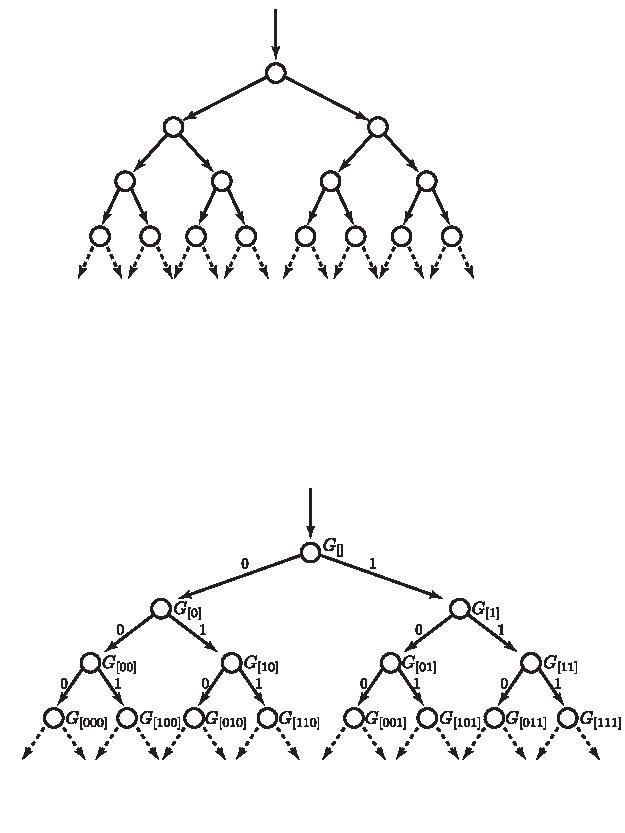
\includegraphics[trim = 4cm 8cm 4cm 8cm, clip, width=5cm]{jtfig/base.pdf}
\vspace{2cm}
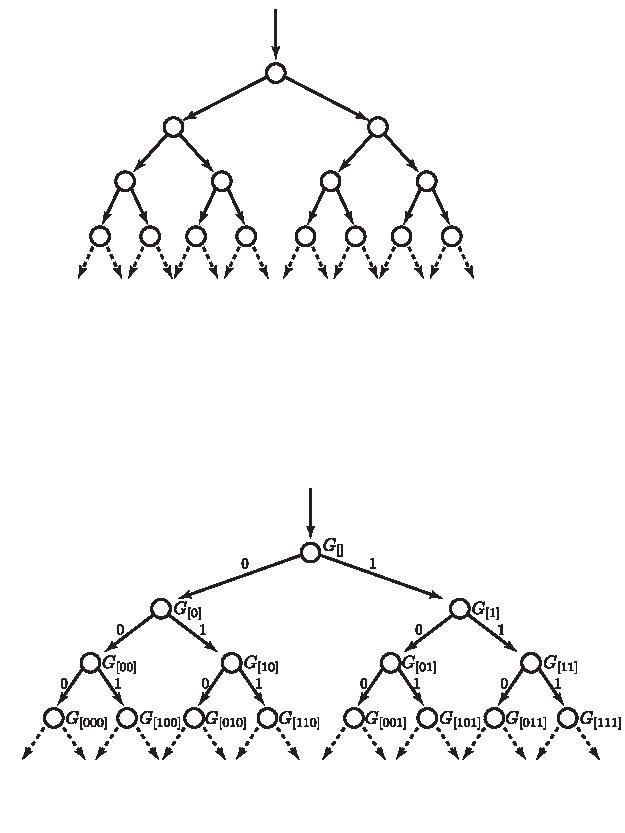
\includegraphics[trim = 2cm 2cm 2cm 10cm, width=8cm]{jtfig/base.pdf}
%\caption{Test perplexity vs.~number of training observations.}
\label{fig: gm_binary_complete}
\end{center}
\end{figure}
}




\comment{
  \frame[t] {%slide 27
 \frametitle{Graphical Model for 110100}
 \begin{figure}[htbp]
\begin{center}
%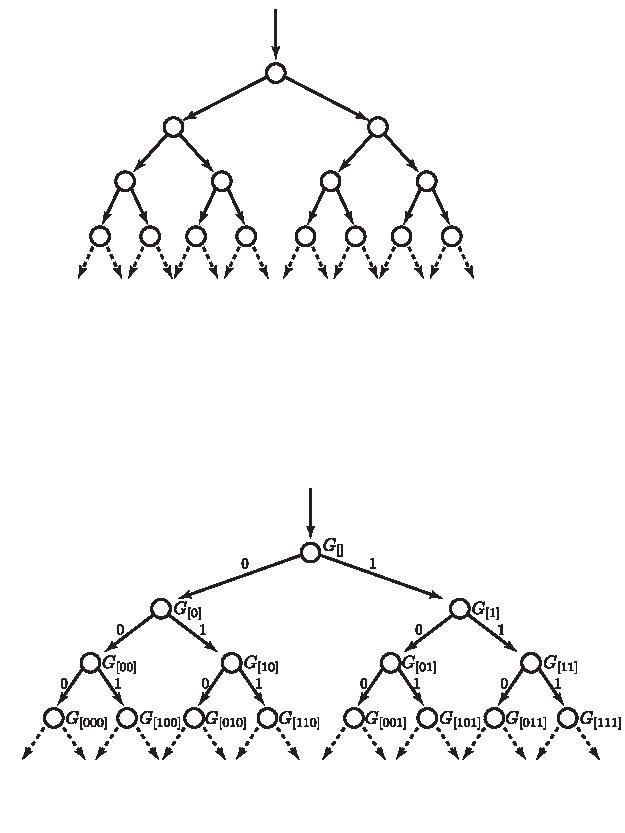
\includegraphics[trim = 4cm 8cm 4cm 8cm, clip, width=5cm]{jtfig/base.pdf}
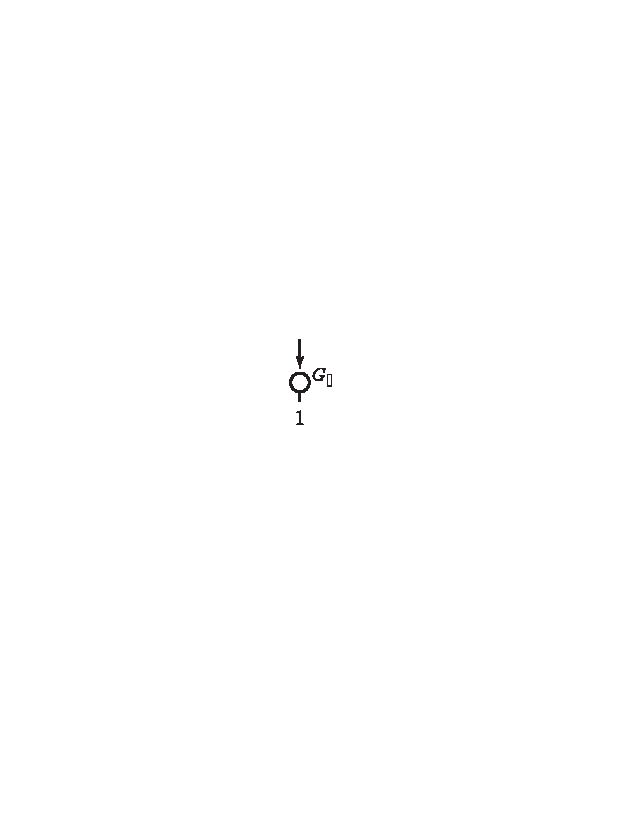
\includegraphics[trim = 2cm 2cm 2cm 6cm, width=8cm]{jtfig/seq_1.pdf}
%\caption{Test perplexity vs.~number of training observations.}
\label{fig: gm_binary_complete}
\end{center}
\end{figure}

 }
 
   \frame[t] {%slide 27
 \frametitle{Graphical Model for 110100}
 \begin{figure}[htbp]
\begin{center}
%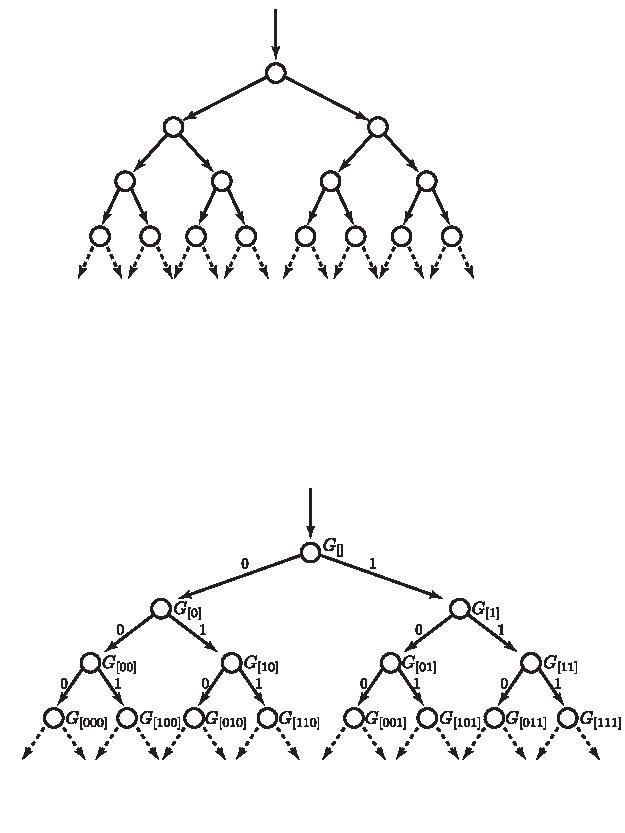
\includegraphics[trim = 4cm 8cm 4cm 8cm, clip, width=5cm]{jtfig/base.pdf}
\includegraphics[trim = 2cm 2cm 2cm 6cm, width=8cm]{jtfig/seq_2.pdf}
%\caption{Test perplexity vs.~number of training observations.}
\label{fig: gm_binary_complete}
\end{center}
\end{figure}

 }

  \frame[t] {%slide 27
 \frametitle{Graphical Model for 110100}
 \begin{figure}[htbp]
\begin{center}
%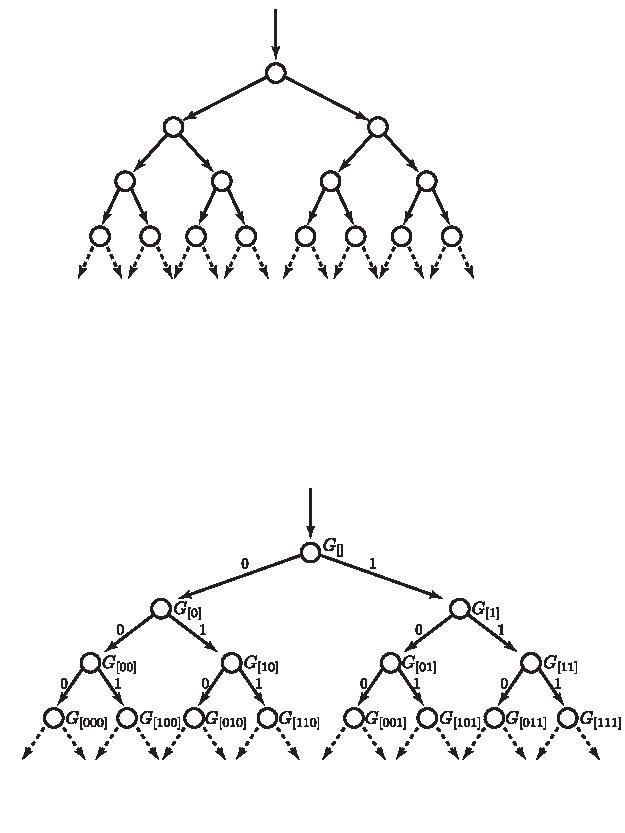
\includegraphics[trim = 4cm 8cm 4cm 8cm, clip, width=5cm]{jtfig/base.pdf}
\includegraphics[trim = 2cm 2cm 2cm 6cm, width=8cm]{jtfig/seq_3.pdf}
%\caption{Test perplexity vs.~number of training observations.}
\label{fig: gm_binary_complete}
\end{center}
\end{figure}

 }
   \frame[t] {%slide 27
 \frametitle{Graphical Model for 110100}
 \begin{figure}[htbp]
\begin{center}
%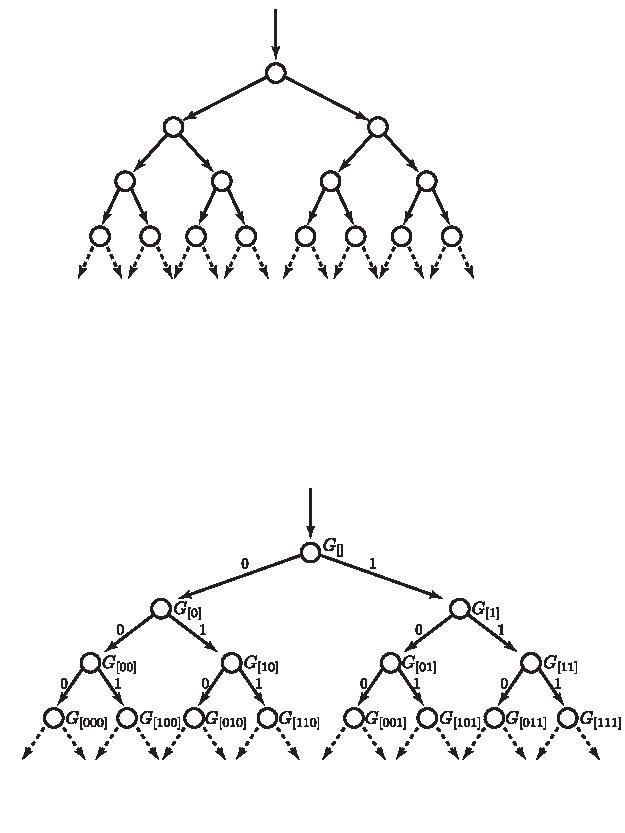
\includegraphics[trim = 4cm 8cm 4cm 8cm, clip, width=5cm]{jtfig/base.pdf}
\includegraphics[trim = 2cm 2cm 2cm 6cm, width=8cm]{jtfig/seq_4.pdf}
%\caption{Test perplexity vs.~number of training observations.}
\label{fig: gm_binary_complete}
\end{center}
\end{figure}

 }
   \frame[t] {%slide 27
 \frametitle{Graphical Model for 110100}
 \begin{figure}[htbp]
\begin{center}
%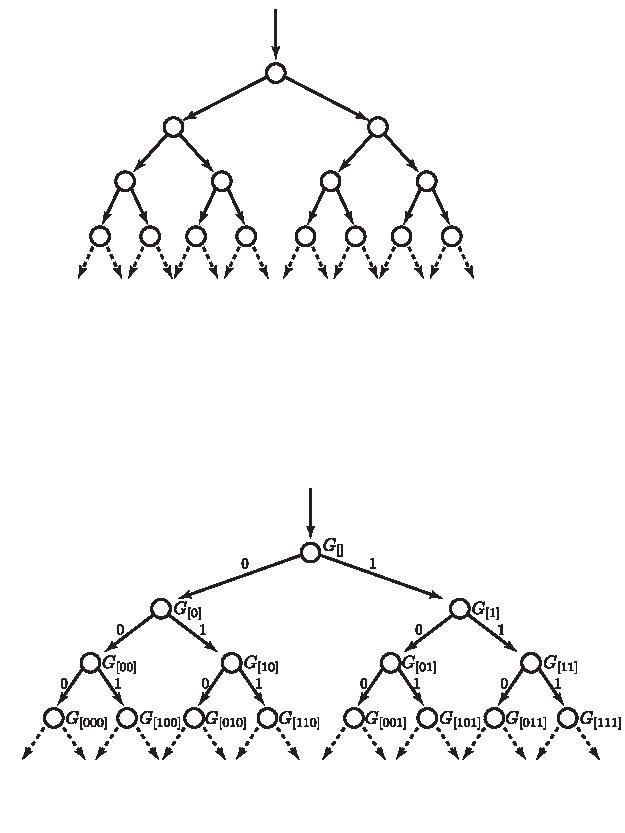
\includegraphics[trim = 4cm 8cm 4cm 8cm, clip, width=5cm]{jtfig/base.pdf}
\includegraphics[trim = 2cm 2cm 2cm 6cm, width=8cm]{jtfig/seq_5.pdf}
%\caption{Test perplexity vs.~number of training observations.}
\label{fig: gm_binary_complete}
\end{center}
\end{figure}

 }
 }
 
  \subsection{Binary sequence memoizer for  sequence 110100}
   \frame[t] {%slide 27
 \begin{figure}[htbp]
\begin{center}
%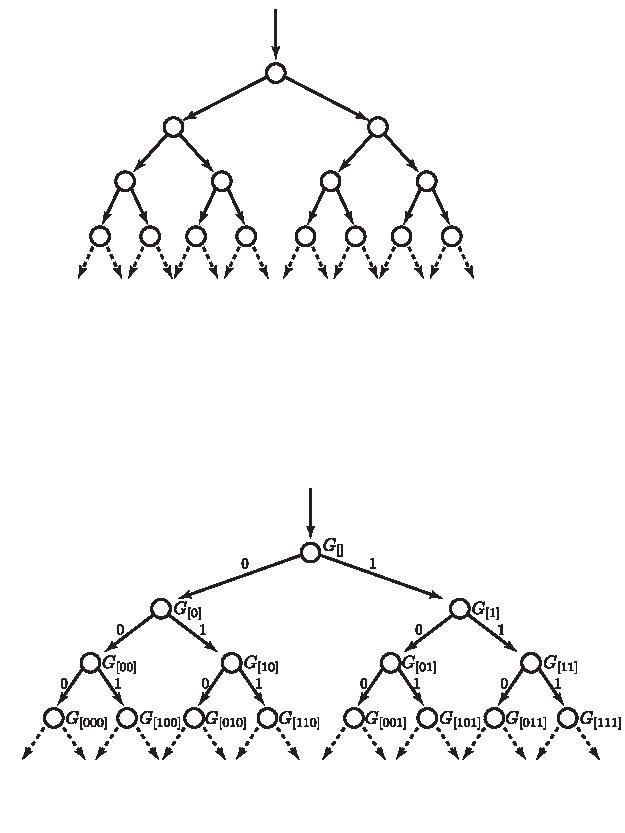
\includegraphics[trim = 4cm 8cm 4cm 8cm, clip, width=5cm]{jtfig/base.pdf}
\includegraphics[trim = 2cm 2cm 2cm 6cm, width=8cm]{jtfig/seq_6.pdf}
%\caption{Test perplexity vs.~number of training observations.}
\label{fig: gm_binary_complete}
\end{center}
\end{figure}

 }

\begin{frame}[t] \frametitle{}
PY process properties exploited by linear space sequence memoizer.
\begin{columns}[c] \column{.5\textwidth} 
\begin{block}{Coagulation \cite{Pitman1999, Ho2006}}
If \[G_2| G_1\sim\py(d_1,0,G_1)\] and \[G_3| G_2\sim\py(d_2,0,G_2)\] then
\[G_3|G_1\sim\py(d_1d_2,0,G_1)\] with $G_2$ marginalized out.
\label{thm:coag}
\end{block}
\column{.5\textwidth} 
\begin{block}{Fragmentation \cite{Pitman1999, Ho2006,Wood2009}}
Suppose
 \[G_3| G_1\sim\py(d_1d_2,0,G_2)\]
 then $G_3$
 can be ``fragmented'' so 
 \[G_2 | G_1 \sim \py(d_1,0,G_1)\]
 and
  \[G_3| G_2\sim\py(d_2,0,G_2)\] 
  if $G_2$ is needed.
\end{block}
 \end{columns}
 \end{frame}

\subsection{Inference, crazy-high level overview}
  \frame[t] {%slide 9
$\EE[\Gu(s)]$
is a recursively defined expectation over a set of random counts
\[\{N(\ubf's'),M(\ubf's')\}_{\ubf'\in\cctx, s'\in\Sigma}\]
which have properties $M(\ubf's') \leq N(\ubf's')$ and $N(\data_{1:i}x_{i+1}) \geq 1 \; \forall \; i$
\begin{block}{}
\vspace{-.5cm}
\[\EE[\G_\context(s)]
= \EE\left[
\frac{N(\context s)-\disc_{\context} M(\context s) + \left(\disc_{\context}\sum_{s'\in\Sigma}  M(\context s')\right) \G_\parent(s)}{\sum_{s'\in\Sigma} N(\context s')}\right]
\]
 \end{block}
The counts
\[\{N(\ubf's'),M(\ubf's')\}_{\ubf'\in\cctx, s'\in\Sigma}\]
are sampled using sequential Monte Carlo or Markov chain Monte Carlo sampling methods.
}
\section{Experiments}


\subsection{Compression}
\frame[t]
{
\begin{block}{}
\begin{table}[t]
    \begin{center}
    \setlength{\tabcolsep}{1.3mm}
\begin{tabular}{l||r|c|c|c|c}
%\hline
%\multicolumn{2}{|c||}{} & \multicolumn{2}{c||}{SM} &
%\multicolumn{2}{|c|}{PPM} & CTW\\\hline
\textbf{Model} & SM & PPM & CTW & bzip2 & gzip \\\hline
%File          &  Size  &    1PF    &    UKN    &   PPM* &    PPMZ  &  CTW  \\\hline 
%\hline
%bib           & 111261 &    1.73   &{\bf 1.72}  &   1.91 &    1.74  &  1.83 \\\hline
%book1         & 768771 &{\bf 2.17}  &    2.20   &   2.40 &    2.21  &  2.18 \\\hline
%book2         & 610856 &{\bf 1.83}  &    1.84   &   2.02 &    1.87  &  1.89 \\\hline
%geo           & 102400 &{\bf 4.40}  &    4.40   &   4.83 &    4.64  &  4.53 \\\hline
%news          & 377109 &{\bf 2.20}  &    2.20   &   2.42 &    2.24  &  2.35 \\\hline
%obj1          & 21504  &{\bf 3.64}  &    3.65   &   4.00 &    3.66  &  3.72 \\\hline
%obj2          & 246814 &    2.21   &{\bf 2.19}  &   2.43 &    2.23  &  2.40 \\\hline
%paper1        & 53161  &    2.21   &{\bf 2.20}  &   2.37 &    2.22  &  2.29 \\\hline
%paper2        & 82199  &{\bf 2.18}  &    2.18   &   2.36 &    2.21  &  2.23 \\\hline
%pic           & 513216 &    0.77   &    0.82   &   0.85 &{\bf 0.76} &  0.80 \\\hline
%progc         & 39611  &    2.23   &{\bf 2.21}  &   2.40 &    2.25  &  2.33 \\\hline
%progl         & 71646  &    1.44   &{\bf 1.43}  &   1.67 &    1.46  &  1.65 \\\hline
%progp         & 49379  &    1.44   &{\bf 1.42}  &   1.62 &    1.47  &  1.68 \\\hline
%trans         & 93695  &    1.21   &{\bf 1.20}  &   1.45 &    1.23  &  1.44 \\\hline \hline
%\textbf{avg.} &        &{\bf 2.12}  &    2.12   &   2.34 &    2.16  &  2.24 \\\hline
\textbf{Average bits / byte}      &{\bf 1.89}   & 1.93  &  1.99 & 2.11 & 2.61 \\%\hline
\end{tabular}
\end{center}
\label{table:results}
\end{table}
\end{block}
Compression performance\footnote{The results for unbounded-length context PPM is from 
\cite{Cleary1997b}. The results for CTW is from \cite{Willems2009}.   The
bzip2 and gzip results come from running the corresponding standard unix
command line tools with no extra arguments.} in terms of weighted average log-loss
\[\ell(\xbf_{1:N}) = -\frac{1}{N}\sum_{i=1}^N \log_2 \EE[G(x_i|\xbf_{1:i-1})]\]
(average bits per byte under optimal entropy encoding, lower is better) for
the Calgary corpus.


}


\subsection{Language modeling}
\frame[t]
{
\begin{block}{}
 \begin{table}
\begin{center}
\begin{tabular}[t]{lcc}
\hline
{\small Source } & {\small Perplexity\footnote{perplexity = $2^{\mathrm{log\; loss}}$}} \\
\hline
{\small Bengio et al.\ \cite{Bengio2003} }& 109.0 \\
%{\small Mnih \& Hinton \cite{Mnih:NIPS08} } & 112.1 \\
{\small Mnih et al.\ \cite{Mnih2009}} & \phantom{0}83.9\\
\hline
{\small 4-gram Interpolated Kneser-Ney \cite{Chen1999} }& 106.1 \\
{\small 4-gram Modified Kneser-Ney \cite{Chen1999} }& 102.4 \\
{\small 4-gram Hierarchical PYP \cite{Teh2006} } & 101.9 \\
{\small Sequence Memoizer} \cite{Wood2009}& \phantom{0}96.9\\
\hline
\end{tabular}
\end{center}
 %It has
 %been reported that the aspects of the data that are modelled by these two
 %distinct classes of models complement each other, so that even higher perfomance
 %can be achieved by combining both types of models.
 % The sequence memoizer outperforms fixed depth smoothing $n$-gram models but is bettered by a more computationally complex model on this data.  }
\label{table:ap_perplexities}
\end{table}
\end{block}
Language models of an Associated Press news corpus (lower perplexity is better).  Interpolated and
 modified Kneser-Ney are state-of-the-art language models.  Provided for comparison are 
 the results for the models of Bengio et al.\ and Mnih et al.\ which belong to
 a different class of models that learn word representations from data. 
}

\frame[t]
{
\begin{figure}
    \includegraphics[width=.85\columnwidth]{cacm_figs/lm_results}
    \label{fig:sm_vs_ngram}
\end{figure}
 SM  versus $n^{\textrm{th}}$ order Markov models with hierarchical PYP priors 
%    $n$-gram model (solid line)
    as $n$ varies.  In red is computational
    complexity. % (for both the sequence 
%    memoizer (dashed line) and a smoothing $n$-gram model (solid line).
    %For this four million word New York Times corpus, as $n$ passes 4, the memory complexity of the Markov models grows larger than that of the sequence
   % memoizer, yet, the SM model yields modeling
   % performance that is better than all Markov models regardless of their order. %the limit of an $n$-gram as $n\rightarrow\infty$.
  %  This suggests that for $n\ge 4$ the SM model is to be preferred: it
  %  requires less space to store yet results in a comparable if not better
  %  model.
}

\section{Demonstration}
\subsection{Compressor based on the sequence memoizer}
\frame[t]
{
A general purpose streaming lossless compressor (``deplump'') built on the sequence memoizer  is available for demonstration at
  \begin{itemize}
  \item \href{http://www.deplump.com/}{http://www.deplump.com/} 
  \begin{itemize}
\item    \href{http://www.deplump.com/LookupStatistics}{real time performance} 
\end{itemize}
\end{itemize}
Source code for the sequence memoizer is downloadable from 
\begin{itemize}
  \item  \href{http://www.sequencememoizer.com/}{http://www.sequencememoizer.com/} 
  \end{itemize}
}



%\section{References}

\subsection{Bibliography}
\bibliographystyle{plainnat}
	\begin{frame}[t,allowframebreaks]{}

\bibliography{../../papers/uber}
\end{frame}

\end{document}
